

\documentclass[tikz,border=10pt]{standalone}
%\documentclass[crop, tikz]{standalone}

\usepackage{tikz}

\begin{document}
	
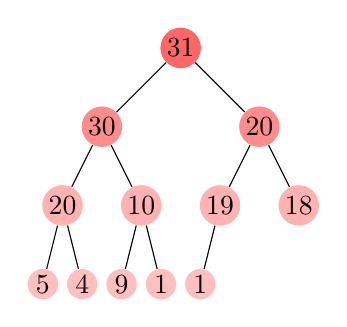
\begin{tikzpicture}
[level distance=10mm,
every node/.style={fill=red!60,circle,inner sep=1pt},
level 1/.style={sibling distance=20mm,nodes={fill=red!45}},
level 2/.style={sibling distance=10mm,nodes={fill=red!30}},
level 3/.style={sibling distance=5mm,nodes={fill=red!25}}]
\node {31}
child {node {30}
	child {node {20}
		child {node {5}}
		child {node {4}}
	}
	child {node {10}
		child {node {9}}
		child {node {1}}
	}
}
child {node {20}
	child {node {19}
		child {node {1}}
		child[missing]
	}
	child {node {18}}
};
\end{tikzpicture}
	
\end{document}
